\documentclass[11pt,a4paper,oneside]{article}
\usepackage{fullpage}
\usepackage{graphicx}
\usepackage{amsmath}
\usepackage{url}

\begin{document}

\title{DISPHOTN v.0.1: User's Guide\\{\small v. 0.1}}
\maketitle
\newpage
\tableofcontents
\newpage

\section{Introduction}
DISPHOTN is a little software for the computation of the eigenfrequencies of the electromagnetic field in a 2D or 3D periodic structure composed of free-space, dielectrics and metals obeying the Lorentz permittivity model. The theoretical model underlying the calculation is based on a description of the problem using auxiliary mechanical fields that keep track of the electron response.

\section{Installation}
The program relies on the combination of the libraries {\tt ARPACK} and {\tt PARDISO} to perform simulations. These libraries, in turn, depends on {\tt LAPACK} and {\tt BLAS}. Moreover, since the language used for the libraries is {\tt FORTRAN}, a suitable compiler should be used to compile those libraries. Once all the libraries required are obtained, the program can be compiled. Using the {\tt gcc} compiler, the command issued could be:

{\tt gcc -c disphotn.c libpardiso.so libarpack.a lapack.a blas.a -lgfortran -lgomp -o disphotn}

This command compiles the C file and links the required libraries, producing the output binary file {\tt disphotn}. Note that the {\tt PARDISO} library is a dynamic library, and therefore must be made available to the program at runtime (e.g. in {\tt /usr/lib}).
The required packages can be found at the following addresses:
\begin{itemize}
\item {\tt ARPACK}: \url{http://www.caam.rice.edu/software/ARPACK/}
\item {\tt PARDISO}: \url{http://www.pardiso-project.org/}
\item {\tt LAPACK} and {\tt BLAS}: these software packages should be included in the {\tt ARPACK} package.
\end{itemize}

\section{{\tt PARDISO} License}
{\tt PARDISO} is proprietary software, and is available only as a precompiled library. A valid license for {\tt PARDISO} must be obtained, and the license file {\tt pardiso.lic} must be placed in the same directory as the executable file. Please see {\tt PARDISO}'s website ( \url{http://www.pardiso-project.org/} ) for more information, and to obtain a license.

\section{Getting Started}
To perform a typical simulation, two files must be provided by the user. A {\it configuration file}, that contains all the information and the parameters required by the simulation, and a {\it mesh file}, containing the spatial discretization (the mesh). The configuration file name is specified either as an argument in the command line, as an absolute or relative path, or is asked by the program at run-time. All the other informations (including the mesh file name) are contained in the configuration file.

\subsection{The Configuration File}
In the configuration file, the parameters required by the software must be specified. A configuration file for DISPHOTN is a simple plain text file that looks like this:
\begin{center}
  \begin{tabular}{| l | l |}
    \hline
   	1 & {\tt \# Comment}\\
	2 & {\tt parameter-name parameter-value}\\
	3 & {\tt flag-name	\qquad	 \# Other comment}\\	
	4 & {\tt sequence-name val1 val2 val3}\\
    \hline
  \end{tabular}
\end{center}

The character \# identifies a comment in the file. Everything after the \# character will be ignored by the program. The second line
shows how a parameter can be defined: the parameter name, space, and the paramenter value. Note that DISPHOTN recognizes numbers written both in decimal and in scentific notation. As an example, to set the parameter \texttt{sigmar}, one may write: \texttt{sigmar 102} or, equivalently, \texttt{sigmar 1.02e+2}.


Flags are boolean parameters. If the configuration file contains the name of the flag, the flag itself is set to \textit{true}, otherwise it is defaulted to \textit{false}. Sequences are lists of values with a certain order. The values are specified after the sequence name, leaving a blank space between them. The maximum number of values for a sequence is hardcoded to 300. Note that if you specify a parameter or a sequence name without writing any value, an error may occur. The following table presents the keywords that can be used in a configuration file:

\newpage
\begin{center}
  \begin{tabular}{| l | l | l | p{230pt} |}
    \hline
   	Keyword & Type & Data Type & Usage \\ \hline
	{\tt meshfile} & P & String & {\bf Required.} Specifies the mesh file to be used in the simulation.  The value can be either a relative or an absolute path. \\ \hline
	{\tt nev} & P & Integer & {\bf Required.} The number of eigenfrequencies requested. \\ \hline
	{\tt a1} & S & Float & {\bf Required.} The first Bravais lattice vector. Only the first 2 (for 2D problems) or 3 (for 3D problems) values of the sequence are considered.\\ \hline
	{\tt a2} & S & Float & {\bf Required.} The second Bravais lattice vector. \\ \hline
	{\tt a3} & S & Float & {\bf Required. 3D only.} The third Bravais lattice vector. \\ \hline
	{\tt kx} & S & Float & The sequence of values for the x component of the {\bf k} vector. The three sequences {\tt kx}, {\tt ky} (and {\tt kz}) must have the same number of elements. \\ \hline
	{\tt ky} & S & Float & The sequence of values for the y component of the {\bf k} vector. \\ \hline
	{\tt kz} & S & Float & {\bf 3D only.}  The sequence of values for the z component of the {\bf k} vector. \\ \hline
	{\tt xperiodic} & F &  & Set this flag to impose Bloch periodicity along the {\bf a1} direction. \\ \hline
	{\tt yperiodic} & F &  & Set this flag to impose Bloch periodicity along the {\bf a2} direction. \\ \hline
	{\tt zperiodic} & F &  & {\bf 3D only.} Set this flag to impose Bloch periodicity along the {\bf a3} direction. \\ \hline
	{\tt zperiodic} & F &  & {\bf 3D only.} Set this flag to impose Bloch periodicity along the {\bf a3} direction. \\ \hline
	{\tt ncv} & P & Integer & Number of Arnoldi vector used by {\tt ARPACK}. If not specified, it is defaulted to 8*{\tt nev}. Please see {\tt ARPACK} documentation for more information. \\ \hline
	{\tt sigmar} & P & Float & The real part of the eigenvalue shift (the normalized target frequency around which look for	eigenvalues). The default value is zero, however, due to the nature of the problem, a nonzero shift should always be specified. \\ \hline
	{\tt sigmai} & P & Float & The imaginary part of the eigenvalue shift. Usually it is better to leave this value zero.\\ \hline
	{\tt dielectric-domains} & S & Integer & The domains corresponding to a dielectric material. Each domain should appear only once. \\ \hline
	{\tt epsilon} & S & Float & The relative permittivity for the domains specified in the sequence {\tt dielectric-domains}. This sequence and the {\tt dielectric-domains} sequence must have the same length.  \\ 
    \hline
  \end{tabular}
\end{center}
\newpage
\begin{center}
  \begin{tabular}{| l | l | l | p{230pt} |}
    \hline
	Keyword & Type & Data Type & Usage \\ \hline
	{\tt metal-domains} & S & Integer & The domains corresponding to a metallic material. Note that the same domain may appear more than once in the sequence. In this case, the domain will be modeled with a multi-pole Lorentz model. \\ \hline
	{\tt omega0} & S & Float & The resonance frequency for the domains specified in the sequence {\tt metal-domains}.  \\ \hline
	{\tt omegap} & S & Float & The plasma frequency for the domains specified in the sequence {\tt metal-domains}. The last three sequences must have the same length. Note that a domain cannot appear both in the {\tt metal-domains} and the {\tt dielectric-domains} sequences. \\ \hline
	{\tt solver} & P & Integer & Specifies the solver used by {\tt PARDISO}. 0 = iterative solver, 1 = direct solver (default). Please see {\tt PARDISO} documentation for more information. \\ \hline
	{\tt bandsfile} & P & String & The output file in which to save the computed eigenfrequencies. \\ \hline
	{\tt modesfile} & P & String & The output file in which to save the electric field configuration. \\ \hline
	{\tt hfieldfile} & P & String & {\bf 2D only.} The output file in which to save the reconstructed magnetic field $H_z$. \\ \hline
	{\tt xgrid} & P & Integer & The size of the interpolation grid on the a1 direction. \\ \hline
	{\tt ygrid} & P & Integer & The size of the interpolation grid on the a2 direction. \\ \hline
	{\tt zgrid} & P & Integer & {\bf 3D only.} The size of the interpolation grid on the a3 direction. The default values for each grid size is 21. \\ \hline
	{\tt gridfile} & P & String & A file containing the points on which the electric field should be interpolated. Please see the section "Grid File" for more information. Note that setting this parameter overrides the values of the xgrid, ygrid and zgrid parameters. \\ \hline
	{\tt penalty} & P & Float & {\bf 2D only.} Penalty for the imposition of interface condition. The default value is 0.7. Please see the "Penalty" section for more information. \\ \hline
    \hline
  \end{tabular}
\end{center}

\newpage

\subsection{Parameters}
An extensive description of some parameters follows.
\begin{itemize}
\item {\tt nev}: this parameter specifies the number of eigenfrequencies to compute. The program will look for the eigenfrequencies around the specified shift expressed in the {\tt sigmar} parameter. Note that due to the nature of the problem
\end{itemize}


\subsection{Mesh File}
DISPHOTN can read and import text mesh files created with COMSOL Multiphysics 3.5 and newer. The mesh file must follow some rules:
\begin{itemize}
\item The mesh file must be text files ({\tt .mphtxt}). If using COMSOL Multiphysics 4.0 or newer, be sure to export the mesh as text file (not binary file).
\item The recognized element types are only triangles (for 2D problems) and tetrahedra (for 3D problems). Other element types (quad, brick, etc.) are not recognized.
\item The mesh must represent the unit cell of a Bravais lattice. One of the vertex of the unit cell must be in the origin, and the edges must be along the a1, a2, (and a3) vectors. This is very important in order to correctly identify the boundaries.
\item The domain numbers to be specified in the sequences {\tt metal-domains} and {\tt dielectric-domains} are the same used in COMSOL.
\item For periodic structures, the mesh must be EXACTLY the same on the two periodic boundaries. Use the "copy mesh" feature in COMSOL to obtain identical meshes.
\end{itemize}
Figure \ref{fig:2dmesh} presents a correct mesh for a 2D triangular lattice. Note that the values of a1 and a2 vectors, in this case, are $(1, 0)$ and $(0.5, \sqrt{3}/2)$
\begin{figure}[h]
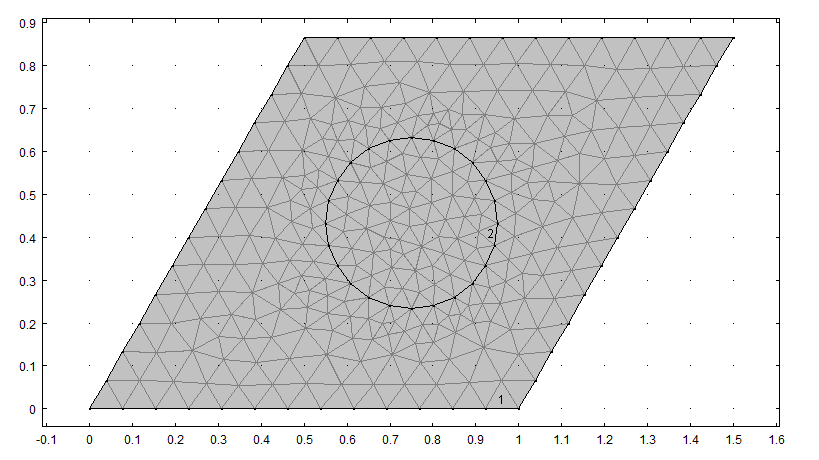
\includegraphics[width=\textwidth]{2dmesh}
\caption{\label{fig:2dmesh}}
\end{figure}

\section{Program Description}

\subsection{Theoretical Background}
The aim of the program is to compute the eigenfrequencies of the electromagnetic field for a periodic structure containing lossless dispersive materials. When computing eigenfrequencies, Maxwell's Equations are usually reformulated as an eigenvalue problem
\begin{equation}
\nabla \times \frac{1}{\mu_0} \nabla \times \boldsymbol{E} = \omega^2 \epsilon_0 \epsilon \boldsymbol{E}.
\label{eq:dielec_eig}
\end{equation}
This eigenvalue problem is in general non-linear for a frequency-dependent dielectric permittivity. However, a linear eigenvalue problem can be obtained in the case of a permittivity that follows the lossless Lorentz's model,
\begin{equation}
\epsilon(\omega)=1+\frac{\omega_{p}^{2}}{\omega_{0}^{2}-\omega^{2}},
\end{equation}
by introducing an auxiliary field. The field is called {\bf P} since it is proportional to the material polarization (i.e. the electron displacement). This field keeps track of the electron response in the metal. Using this formulation, the eigenvalue problem becomes:
\begin{equation}
\omega^{2}\left[
\begin{array}{c}
\boldsymbol{E}\\
\boldsymbol{P}
\end{array}
\right]=\left[
\begin{array}{cc}
\frac{1}{\epsilon_{0}}\nabla\times\frac{1}{\mu_{0}}\nabla\times\bullet+\omega_{p}^{2}\bullet & -\frac{\omega_{0}^{2}}{\epsilon_{0}}\bullet\\
-\omega_{p}^{2}\epsilon_{0}\bullet & \omega_{0}^{2}\bullet
\end{array}
\right]\left[
\begin{array}{c}
\boldsymbol{E}\\
\boldsymbol{P}
\end{array}
\right].
\label{eq:2_fields}
\end{equation}
This formulation is valid in the metallic regions. In the freespace or dielectric regions, the usual eigenvalue problem Eq. \eqref{eq:dielec_eig} can be used.

\subsection{Domain and Boundary Conditions}
Since the program is aimed to the simulation of periodic structure, the domain of the problem is assumed to be an unit cell of a Bravais lattice. This means that it must be spanned by two (2D) or three (3D) linearly independent vectors (the Bravais primitive vectors). As a consequence, the domain must always be a quadrilateral (2D) or a 6-faced polyhedron (3D). This makes easier to compute the photonic bands in a periodic structure. Note that the unit cell may actually contain anything, so even traditional non-Bravais lattices (such as a diamond lattice) can be simulated.

On such cells, two kinds of boundary conditions can be imposed: a Perfect Electric Conductor (PEC) condition, and Bloch Periodic conditions. Opposite boundaries share the same condition type, i.e. both of them are obviously either PEC or periodic. Setting the {\tt x}-, {\tt y}- and {\tt zperiodic} flags in the configuration file imposes the periodicity on the three pairs of boundaries; if the flags are not set, the PEC conditions are enforced.
The PEC condition is simply imposed by setting the tangential component of the electric field to zero on the boundary. The Bloch periodic condition establishes a relation between the field on opposite boundaries, according to Bloch's Theorem:
\begin{equation}
\boldsymbol{E}_{\boldsymbol{k}}(\boldsymbol{x} + \boldsymbol{R})=e^{i\boldsymbol{k\cdot R}}\boldsymbol{E}_{\boldsymbol{k}}(\boldsymbol{x}).
\end{equation}
Using this relation, the value of the field on a boundary is proportional to the value of the field on the opposite boundary, with a phase coefficient dependent on the geometry of the unit cell and the $\boldsymbol{k}$ vector specified by the user.

\subsection{Discretization}
In order to discretize the problem, a Finite-Elements Method (FEM) is used, with edge-element type basis function. The domain of interest is subdivided into a mesh composed of triangles (2D) or tetrahedra (3D). The equations are then enforced in weak form on each mesh element. This transforms the differential eigenvalue problem in a matrix eigenvalue problem. The size of the matrices involved depends on some of the properties of the problem. The base matrix size is the number of edges in the mesh. For each metallic domain specified in the {\tt metal-domains} sequence, the size of the matrix is increased of the number of edges contained in the domain. Note that if the same domain appears more than once in the sequence (for example, to simulate a multi-pole Lorentz model) its edges are counted multiple times. From this total, the number of edges on PEC boundaries must be subtracted, and half of the number of edges on periodic boundaries (since in this last case the field on each edge can be expressed in terms of the field on the opposite edge).

\subsection{Interface Conditions and Penalty}
The use of edge-based elements has some advantages and some disadvantages. The solutions obtained are guaranteed to have null divergence inside each domain, and the tangential continuity of the electric field is automatic. However, the other conditions at the interface (namely, the normal continuity of the dielectric displacement field) are difficultly implemented. The failure in the imposition of correct interface conditions at a metallic interface give rise to spurious modes, localized on the interface itself, that pollute the compute spectrum. To remove these modes, the edges on the interface are treated as if they belong interely to the metallic region; unfortunately, using this method alters the computed eigenfrequencies of the higher order surface modes (the ones more localized on the metallic interface), moving them to higher values. In 2D problems, the {\tt penalty} parameter can be used to tune the interface condition. The default value for this parameter is 0.7; lower values give more correct eigenfrequencies, but values below 0.5 may cause spurious modes to occur. In general, finer meshes give correct eigenmodes even with lower {\tt penalty} values.
If the lowest order surface modes are of interest, and if a sufficiently fine mesh can be used, the {\tt penalty} parameter can be set to a very low value (or zero) in order to obtain correct eigenfrequencies for the first modes. In 3D problems, due to performance reasons, the value of the {\tt penalty} parameter is fixed at 1.

\subsection{Band Structure Computation}
The program is able to compute band structures for a periodic structure. To do so, simply specify the values of the $\boldsymbol{k}$ vector (k-points) at which the eigenfrequencies should be computed. The program will then compute {\tt nev} eigenvalues for each k-point. All the eigenfrequencies and eigenmodes are saved in the results files. Note that the values of the {\tt k} vector are chosen by the user, so they should be chosen accordingly to the geometrical properties of the structure. As an example, to compute the $\Gamma$-X-M-$\Gamma$ band structure for the 2D square lattice spanned by the vectors $(1, 0)$ and $(0, 1)$, the {\tt kx} and {\tt ky} parameters may be specified as follows:

  \begin{tabular}{l}
{\tt kx 0 .2 .4 .6 .8 1 1 1 1 1 1 .8 .6 .4 .2 0} \\
{\tt ky 0  0  0  0  0  0 .2 .4 .6 .8 1 .8 .6 .4 .2 0} \\
  \end{tabular}

Doing so, the program will compute the eigenfrequencies at various k points going from $\boldsymbol{k} = (0,0)$, to $\boldsymbol{k} = (1,0)$, then to $\boldsymbol{k} = (1,1)$, and finally back to $\boldsymbol{k} = (0,0)$.
The value of $\boldsymbol{k}$ affects the periodic boundary conditions. Those kind of conditions, therefore, need to be reimposed at every k-point. Note that if no boundary has a Bloch-type boundary conditions, the values in the {\tt kx} and {\tt ky} sequences are ignored and the simulation will only run once; anyway, the program will not check if the specified k-points are valid for the structure.

\subsection{Eigensolving}
Once the matrices are built and the boundary conditions are imposed, the eigensolver is started. Two external libraries are used in the eigensolving process: the {\tt ARPACK} eigensolver and the {\tt PARDISO} linear system solver. {\tt ARPACK} is an iterative solver that finds an approximation of the eigenvalues and the eigenvector of the matrices. {\tt PARDISO} is a linear system solver used to solve the problem in shift-and-invert mode. These two libraries are chosen in order to reduce the memory consumption and allow the solution of large-scale problems. The user is granted a limited control on the actual eigensolving process. The {\tt ncv} parameter, used by {\tt ARPACK}, specifies the number of Arnoldi vectors to be used. This can affect in various ways the eigensolving; for more information, we refer to {\tt ARPACK}'s documentation. The {\tt solver} parameter is used by {\tt PARDISO} and specifies whether an iterative ({\tt solver} = 0) or direct ({\tt solver} = 1) solver must be used. Once again, we refer to {\tt PARDISO} documentation for more information.

\subsection{Target Frequency}
As mentioned, the parameter {\tt sigmar} specifies a target frequency around which the eigenfrequencies should be computed. The choice of this parameter is of crucial importance in the simulation, directly influencing the eigenmodes found and the computation time. In order to choose the right target frequency, a general knowledge of the problem and the physics involved is needed.
Moreover, the discretization using edge-elements introduces a great number of nonphysical modes with frequency zero and at all the frequencies in which the Lorentz dielectric permittivity vanishes. Since these effectively count as very large eigenvalue clusters, {\tt ARPACK} has problems when trying to compute eigenvalues at those frequencies. Therefore, the parameters {\tt sigmar} and {\tt nev} must be chosen accordingly to avoid trying to compute eigenvalues belonging to those clusters.

\subsection{Postprocessing and Interpolation}
Once the desired number of eigenvectors converged, an usable set of results must be computed. The eigenvectors obtained are the edge-elements coefficients and can be physically interpreted as the value of the fields on each edge in the tangential direction. However, this set of value is of little use, and must be transformed in a more useful form. The program performs an interpolation of the field on a discrete regular grid. The value of the Cartesian components of the field at each grid points are computed using the Finite Elements basis functions. There are two ways to specify an interpolation grid. The first is to use the built-in grid generator, that creates a regular grid of the same shape of the unit cell. The parameters {\tt xgrid}, {\tt ygrid}, and {\tt zgrid} specify the size of the grid in the {\tt a1}, {\tt a2}, and {\tt a3} directions (Note: \underline{not} the Cartesian $x$, $y$ and $z$ directions!). Especially in the case of 3D problems, a large value for this parameters can result in a very large grid, and consequently a long interpolation time. Alternatively, the user may provide a text file containing the grid points on which the interpolation must be carried on. The file name must be specified in the {\tt gridfile} parameter. If this parameter is set, the values of the {\tt x}-, {\tt y}- and {\tt zgrid} parameters are ignored.

\subsection{Grid File}
The grid file is a plain text file. The first (non-empty or non-comment) line must contain a single integer value equal to the number of grid points contained in the file. The following lines must contain the coordinates $x$ $y$ (or $x$ $y$ $z$) of the interpolation points, expressed as floats separated by a blank space. As with the configuration file, the \# character introduces a comment. The filename (as an absolute or relative path) of the grid file must then be specified in the {\tt gridfile} parameter in the configuration file.

\subsection{Results and {\tt MATLAB} functions}
The program produces two series of data as a result of the computation. The eigenfrequencies computed at each k-point are saved in a text file, if a filename is specified in the {\tt bandsfile} parameter. The file consists in a table with {\tt nev} rows and a number of columns equal to the number of k-points required. Each column presents the eigenfrequencies computed for the corresponding k-point.

The computed eigenmodes of the electric field are stored in the {\tt modesfile} file, if specified. For 2D (3D) problems, the first two (three) rows give the coordinates $x$, $y$ and $z$ of the interpolation grid points, separated. Then, the data is organized in a number of blocks equal to the number of k-points. In each block, the first {\tt nev} lines give the interpolated values of the $x$ component for each computed eigenmode at that specific k-point, followed by other {\tt nev} lines containing the $y$ component values, and (for 3D problems), other {\tt nev} lines with the $z$ component values. All the values of the field may be complex.
Some code for {\tt MATLAB} has been provided in order to allow a manipulation and visualization of the results. To import the {\tt bandsfile} (the file containing the computed eigenfrequencies), simply use {\tt MATLAB}'s function {\tt dlmread}. To import the results from the {\tt modesfile}, use the function {\tt disphotn\_extract\_mode\_2d} (or {\tt \_3d}), that extracts the interpolated electric field for the specified eigenmode. For example, one can visualize a vector plot of the electric field of the $i$-th eigenmode of the $j$-th k-point in the following way. First, the grid coordinates and the field values are extracted from the result file:

{\tt [x y fx fy] = disphotn\_extract\_mode\_2d(modesfile,\ nev,\ j,\ i);}

\noindent
and then plotted as a vector plot:

{\tt quiver(x,\ y,\ real(fx),\ real(fy));}

\noindent
For 2D problems, a third set of data is produced. The reconstructed $z$ component of the magnetic field is stored in {\tt hfieldfile}, if specified. The format of this file is the following: it contains a number of blocks equal to the number of k-points, and each block contains {\tt nev} lines. Each line, in turn, contains the value of the $Hz$ component of the magnetic field in each triangle on the mesh. The value can, in general, be complex. The magnetic field is not interpolated in order to take advantage of {\tt MATLAB}'s {\tt pdeplot} function. In MATLAB, first import the mesh with the provided {\tt disphotn\_import\_comsol\_mesh} function:

{\tt [points\ edges\ triangles] =  disphotn\_import\_comsol\_mesh(meshfile);}

\noindent
retrieve the magnetic field value from the result file:

{\tt h = disphotn\_extract\_mode\_h(hfieldfile, nev, k, modn);}

\noindent
and, finally, plot the $Hz$ field:

{\tt pdeplot(points,\ edges,\ triangles,\ \text{'}xydata\text{'},\ real(h));}

\section{Example\label{sec:example}}
The following is an example of a 2D structure that can be simulated using {\tt DISPHOTN}. The structure is a simple square lattice of cylinders, with the ratio between radius and lattice parameter equal to $0.25$. The square lattice with unitary lattice parameter is defined by the primitive vectors $(1, 0)$ and $(0, 1)$. The mesh is represented in Figure \ref{fig:example_mesh}, contained in the file {\tt square\_lattice\_example.mphtxt}. The metal will be described by a Drude model with normalized plasma frequency equal to one. To obtain a Drude model from a Lorentz model, it is necessary to take the limit $\omega_0 \rightarrow 0$; in our simulation, we put $\omega_0 = 0.001$. We will ask the program to compute the complete photonic band diagram ($\Gamma$-X-M-$\Gamma$), finding 16 bands in the region of the lower order surface modes. The resulting configuration file is {\tt square\_lattice\_example.txt}:
\begin{figure}[t]
\begin{center}
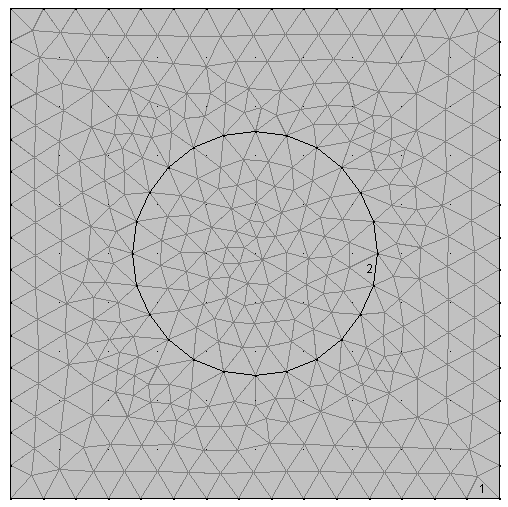
\includegraphics[width=0.7\textwidth]{example.png}
\caption{\label{fig:example_mesh} Mesh for the example problem in Sect. \ref{sec:example}.}
\end{center}
\end{figure}
{\tt \\ \\
\# Sample Configuration File for DISPHOTN. \\
\# Name of the mesh file \\
meshfile square\_lattice\_example.txt \\
\\
\# Geometry of the lattice \\
a1 1 0 \\
a2 0 1 \\
\\
\# Periodicity \\
xperiodic \\
yperiodic \\
 \\
\# Metallic domains and their properties \\
metal-domains 2 \\
omegap 1 \\
omega0 0.001 \\
 \\
\# Band Structure computation \\
kx 0 .2 .4 .6 .8 1 1  1  1  1  1 .8 .6 .4 .2 0 \\
ky 0 0  0  0  0  0 .2 .4 .6 .8 1 .8 .6 .4 .2 0 \\
\\
\# Target Frequency \\
sigmar .6\\
 \\
\# Number of requested eigenfrequencies \\
nev 16\\
\\
\# Output files\\
bandsfile example\_bands.txt\\
modesfile example\_modes.txt\\
hfieldfile example\_hfield.txt\\
}

The simulation is then run by executing {\tt disphotn} and passing the configuration file on the command line or inputting the name when prompted. The program will compute the band diagram, calculating 16 eigefrequencies around the normalized frequency of 0.6, varying the value of the $\boldsymbol{k}$ vector according to the values specified in {\tt kx} and {\tt ky}. At the end of the computation, the resulting eigenfrequencies are saved in the file {\tt example\_bands.txt}. To visualize the band diagram, one can import the data in {\tt MATLAB}:

{\tt bands = dlmread(\text{'}example\_bands.txt\text{'});}

\noindent
and then plot it:

{\tt plot(bands.\text{'},\ \text{'}k.\text{'});}

\begin{figure}
\begin{center}
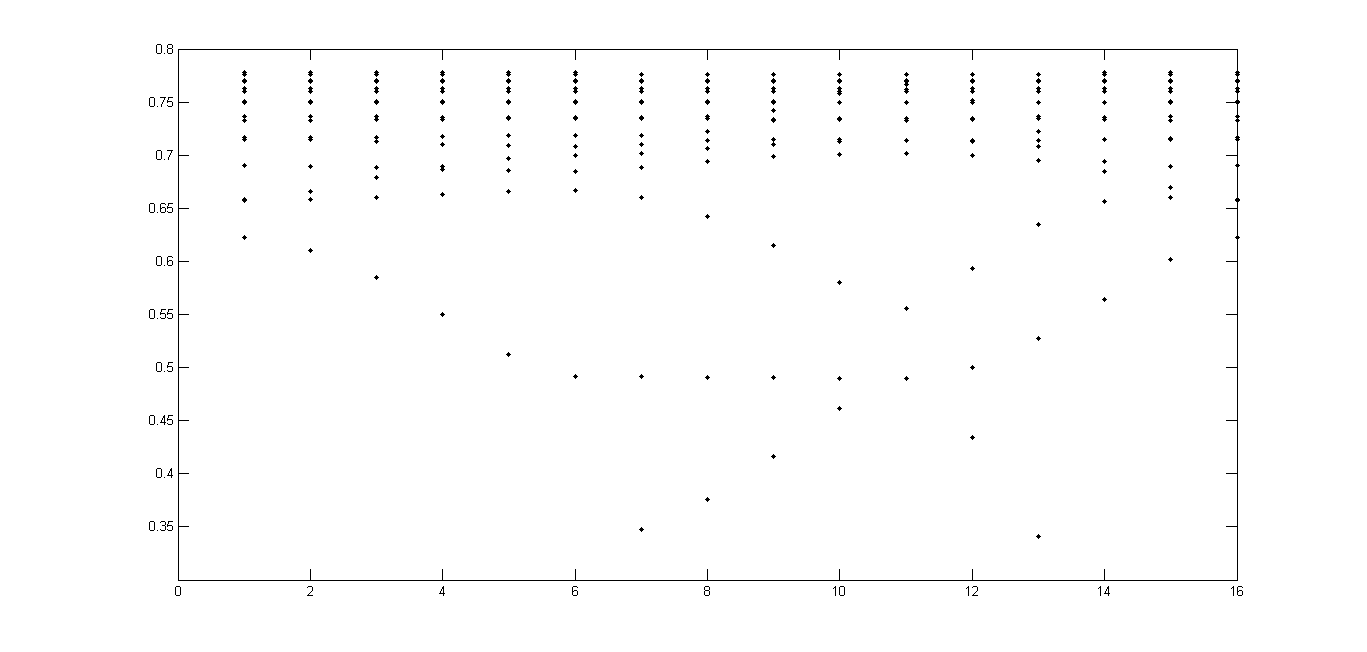
\includegraphics[width=\textwidth]{bands.png}
\caption{\label{fig:bands} The band diagram obtained plotting the results with {\tt MATLAB}.}
\end{center}
\end{figure}

The band plot is presented in Fig. \ref{fig:bands}. As mentioned, due to the correction to spurious modes introduced, the surface plasmon modes (the flat bands) have frequencies higher than the expected convergency frequency ($1/\sqrt{2} \simeq 0.7071$).
The eigenmodes of the magnetic field can be visualized as well, since we are dealing with a 2D problem. First, the mesh file and the $H$ field values must be imported:

{\tt [points\ edges\ triangles] =  disphotn\_import\_comsol\_mesh(\text{'}square\_lattice\_example.mphtxt\text{'});} 


{\tt h = disphotn\_extract\_mode\_h(\text{'}example\_hfield.txt\text{'}, 16, 1, 1);}

\noindent
The two $1$'s in the second command select the first mode of the first k-point. The actual visualization of the mode is carried on using the {\tt pdeplot} function:

{\tt pdeplot(points,\ edges,\ triangles,\ \text{'}xydata\text{'},\ real(h));}

\noindent
The result is reported in Fig. \ref{fig:mode}

\begin{figure}
\begin{center}
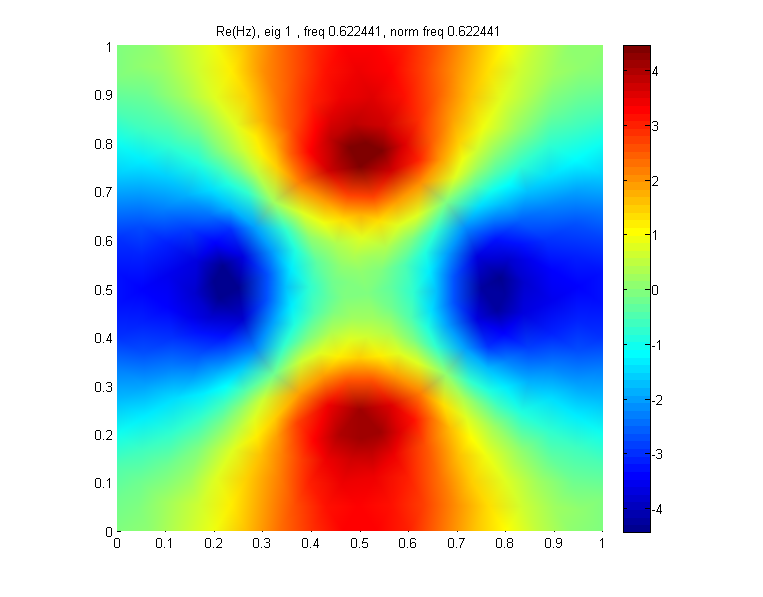
\includegraphics[width=\textwidth]{mode.png}
\caption{\label{fig:mode} Magnetic field plot for the first eigenvalue computed for the first k-point.}
\end{center}
\end{figure}



\end{document}